\chapter{Transfer Learning}
\label{ch:transfer_learnimg}

\begin{remark}{Outline}
	We now present Transfer Learning (TL), a machine learning methodology that aims at creating algorithms that are capable of retaining and reusing previously learned knowledge when getting trained on new, unseen problems. Most of the contributions presented within this dissertation are motivated by TL, therefore, we now introduce the reader to this specific learning paradigm with the goal of providing him/her with all the preliminary knowledge that is necessary for fully understanding the research that will be presented in the coming chapters. We start with a gentle introduction to TL in Sec. \ref{sec:tl_introduction} where we present the main concepts underlying TL and explain why it is desirable to have machine learning models that are transferable. We then show in Sec. \ref{sec:rationale} some practical, high level, examples that visually represent the benefits that come from adopting TL strategies in machine learning. We will then provide more rigorous, mathematical definitions of TL in Sec. \ref{sec:definitions} where we will characterize TL both for supervised learning as for reinforcement learning. In Sec. \ref{sec:literature_review} we thoroughly review how TL has already been studied by the deep learning community, and we will again focus on supervised learning and on reinforcement learning. We end this chapter with Sec. \ref{sec:relevance} where we summarize the most relevant TL concepts that underpin the contributions that will be presented throughout in this dissertation.  
\end{remark}

\section{Introduction}
\label{sec:tl_introduction}


\section{Rationale of Transfer Learning}
\label{sec:rationale}

Before mathematically defining TL we start by building some intuition and visually represent how one can observe the benefits of TL in practice. We assume that we would like to solve a certain task, and that we can choose between two different models: a model that has never dealt with any kind of task before, and a second model, which is identical to the first one with the major difference being that it has already seen a similar task in the past. Because of their different nature, we refer to the first model as a model that will be trained from scratch, and to the second model as a pre-trained model. Ideally, as mentioned in the previous section, we would like the latter model to perform better on the considered task that the first one. Yet, how can we asses if one model is better than the other one? As initially presented by \citet{langley2006transfer} and later generalized by \citet{lazaric2012transfer} we would like the performance of a pre-trained model to result into three possible improvements. If at least one of these improvements is observed while training, we can then consider the pre-trained model to be better than the scratch model. These improvements are the following:
\begin{itemize}
	\item \textcolor{RoyalBlue}{Learning Speed Improvements}: in this scenario the performance between a pre-trained model and a model trained from scratch is identical by the time training is finished, however when this kind of improvement appears we observe that the pre-trained model converges faster than the model trained from scratch. An example of this TL improvement is presented in the first plot of Fig. \ref{fig:tl_examples}. The goal is to train a model such that by the end of training its performance reaches a value of $200$. We can clearly see that both models manage to converge to this desired performance value, but that the pre-trained model manages to converge already after $\approx 50$ training iterations, whereas the model trained from scratch requires more than $200$ training iterations to perform similarly. Also note that the performance of both models at the beginning of training is identical, with both models starting with an initial performance of $\approx20$.

	\item \textcolor{RoyalBlue}{Jumpstart Improvements}: similarly to the previous case, also in this scenario there are no significant differences between the performance of a pre-trained model and the performance of a random model by the end of training. However this changes when we consider the very first training iteration. If jumpstart improvements appear, we can usually observe that when both models start their training process, the performance of the pre-trained model is much closer to the one that will be obtained by the end of training than the one of the scratch model. We visually report an example of this scenario in the third plot of Fig. \ref{fig:tl_examples}. In this case the goal is to train a model such that by the end of training its performance will be of $\approx -100$. We can clearly see that by the end of training both models are able to successfully achieve this goal, but that at the very first training iteration, the performance of the pre-trained model is significantly closer to the desired final performance ($\approx -250$) than the one of the scratch model ($\approx -450$). 
	\item \textcolor{RoyalBlue}{Asymptotic Improvements}: when this TL improvement appears, the final performance of a pre-trained model is significantly higher than the one of a model trained from scratch. It is worth noting that similarly to what happens when learning speed improvements are observed, also in this case the performance of both models is identical when training begins, and that this TL improvement only presents itself after several training iterations. A visualization of this TL improvement can be observed in the last plot of Fig. \ref{fig:tl_examples} where we can observe that for the first $\approx 20$ training iterations there are no differences in terms of performance between a pre-trained model and a model trained from scratch. However the more training iterations are performed, the more the pre-trained model starts outperforming the model trained from scratch, reaching a final performance that is almost twice as good by the $100\text{th}$ training iteration.
\end{itemize}

\begin{figure}[ht!]
  \begin{tikzpicture}[scale = 0.65]
      \begin{axis}[
	name=ax1,
      	grid style={dashed,gray},
      	grid = both, 
      	tick style=black,
	title=Learning Speed Improvements,
        xlabel=Training Iterations,
        ylabel=Performance,
      ]


      \addlegendentry{Pre-trained Model} 
      \addlegendentry{Scratch Model}  
      
      \addplot [ultra thick, blue, mark=.] table [y=Transfer, x=episodes]
      {./Results/Chapter03/logs/speed_improvements.txt};
       \addplot [ultra thick, orange, mark=.] table [y=No-Transfer, x=episodes]
      {./Results/Chapter03/logs/speed_improvements.txt};
     
      \legend{}

      \end{axis}

      \begin{axis}[
      	at={(ax1.south east)},
	xshift=2cm,
	grid style={dashed,gray},
      	grid = both, 
      	tick style=black,
	title=Jumpstart Improvements,
        xlabel=Training Iterations,
        ylabel=Performance,
      ]



      \addlegendentry{Pre-trained Model} 
      \addlegendentry{Scratch Model}  
      
      \addplot [ultra thick, blue, mark=.] table [y=Transfer, x=episodes]
      {./Results/Chapter03/logs/jumpstart_improvements.txt};
       \addplot [ultra thick, orange, mark=.] table [y=No-Transfer, x=episodes]
      {./Results/Chapter03/logs/jumpstart_improvements.txt};
     
      \legend{}

      \end{axis}


      \begin{axis}[
	at={(ax1.south east)},
	xshift=-2cm,
      	yshift=-8cm,
	grid style={dashed,gray},
      	grid = both, 
      	tick style=black,
	title=Asymptotic Improvements,
        xlabel=Training Iterations,
        ylabel= Performance,
	legend columns=4, 
        legend style={font=\Large, at={(-0.3,-0.3,-0.4)},anchor=north west,legend columns=3},
      ]


      \addlegendentry{Pre-trained Model} 
      \addlegendentry{Scratch Model}  
 
      \addplot [ultra thick, blue, mark=.] table [y=Transfer, x=episodes]
      {./Results/Chapter03/logs/asymptotic_improvements.txt};
      \addplot [ultra thick, orange, mark=.] table [y=No-Transfer, x=episodes]
      {./Results/Chapter03/logs/asymptotic_improvements.txt};
       
      \end{axis}
	\end{tikzpicture}
	\caption{A visualization of the three possible desired outcomes that can come from adopting Transfer Learning strategies as initially defined by \citet{langley2006transfer} and later by \citet{lazaric2012transfer}.}
	\label{fig:tl_examples} 
\end{figure}



While all the improvements presented in Fig. \ref{fig:tl_examples} are all highly desirable, it is  worth noting that some of them can be more preferable than others. In fact, the potential benefits of TL highly depend from the problem at hand. As an example, let us consider a training situation where the main goal is that of minimizing the overall training time of a model. In this particular case, jumpstart and learning improvements are more desirable than asymptotic improvements, since the latter improvement might not result into a model that converges to a desired solution faster. On the other hand, if the main objective is that of training a model which performs as best as possible, than evidently, asymptotic improvements are preferred. It is also worth noting that the examples presented in Fig. \ref{fig:tl_examples} are not mutually exclusive, and that the benefits of TL can present themselves as a combination of improvements, rather than in the form of a single, isolated, improvement. 

Now that we have introduced the key ideas behind TL, and presented why adopting TL training strategies is beneficial we move to formally characterizing this machine learning paradigm both from a supervised learning perspective as from a reinforcement learning one.  


\section{Mathematical Definitions}
\label{sec:definitions}

As is common throughout this thesis we start by focusing on the supervised learning case.

\subsection{Supervised Learning}
The first two definitions that we provide are borrowed from \citet{zhuang2020comprehensive} and are the ones of \textcolor{RoyalBlue}{domain} and \textcolor{RoyalBlue}{task}. The first one is defined as follows:
\begin{definition}
	A domain $\mathcal{D}$ is the combination between an input space $\mathcal{X}$ and a marginal distribution $P(X)$, $\mathcal{D} = \{\mathcal{X},P(X)\}$ where $X$ denotes an instance set defined as $X=\{\vec{x}|\vec{x_i}\in \mathcal{X}, i =1, \cdots, n \}$.
\end{definition}
Examples of domains can be natural images, time-series data, biomedical markers and so on. In supervised learning we know that each domain is associated to its respective task, which is representative of the problem we would like to solve. A task is defined as follows:
\begin{definition}
	A task $\mathcal{T}$ consists of a label space $\mathcal{Y}$ and a decision function $f$, i.e., $\mathcal{T}=\{\mathcal{Y},f\}$. The decision function $f$ is implicit and can only be learned by sampling data from $\mathcal{X}$ which comes in the form of $\{x_i,y_i\}$ pairs where $x_i\inX$ and $y_i \in \mathcal{Y}$.
\end{definition}
Examples of possible decision functions $f$ can be classifiers which categorize natural images in their respective classes, or regressors that are able to predict future values in a time-series. 
The key concept underlying TL is that, differently from the common supervised learning scenario
where the only information that is available to a model are one domain and one task, we now have access to at least two domains. The one that corresponds to the task we would like to solve, called the \textcolor{RoyalBlue}{target-domain} $\mathcal{D}_T$, and an additional, possibly related, domain that comes with the name of the \textcolor{RoyalBlue}{source-domain} $\mathcal{D}_S$. With all these concepts in place we can now define \textcolor{RoyalBlue}{Transfer Learning} as:
\begin{definition}
Given one, or more, observations corresponding to $m^s \in \mathds{N}^{+}$ source domain(s) and tasks(s) (i.e., $\{(\mathcal{D}_{S}_{i}, \mathcal{T}_{S}_{i}|i=1\cdots,m^s)\})$ and some additional observation(s) about $m^T \in \mathds{N}^{+}$ target domain(s) and task(s) (i.e. $\{(\mathcal{D}_{T}_{j},\mathcal{T}_{T}_{j}|j=1,\cdots,m^T)\})$, transfer learning utilizes the knowledge implied in the source domains to improve the performance of the learned decision functions $f^{T}_j(j=1,\cdots,m^T)$ on the target domain(s).
\end{definition}
As pointed out by \citet{pan2009survey} the condition that the source and the target domains might be different $\mathcal{D}_S \neq \mathcal{D}_T$ implies that either their respective input spaces are different as well $\mathcal{X}_S\neq\mathcal{X}_T$, or that their corresponding marginal distributions are different $P_s(X)\neq P_T(X)$. Similarly, if the tasks are different instead $\mathcal{T}_S\neq\mathcal{T}_T$, then either one between the output spaces, or the conditional distributions has to be different ($\mathcal{Y}_S\neq\mathcal{Y}_T$ or $P(Y_S|X_S)\neq P(Y_T|X_T))$.

Based on the consistency between the source and target input spaces $\mathcal{X}$, and the respective output spaces $\mathcal{Y}$, one can categorize TL into three following settings.

\paragraph{Inductive Transfer Learning}
This TL scenario is characterized by the fact that the target task $\mathcal{T}_T$ is different from the source task $\mathcal{T}_S$, while the source domain $\mathcal{D}_S$ and the target domain $\mathcal{D}_T$ might, or might not, be similar. As originally presented in \cite{pan2009survey} we define inductive transfer learning as:
\begin{definition}
	Given a source domain $\mathcal{D}_S$ and a learning task $\mathcal{T}_S$, and a target domain $\mathcal{D}_T$ and a learning task $\mathcal{T}_T$, inductive transfer learning aims to help improving the target predictive function $f_T(\cdot)$ in $\mathcal{D}_T$ by using the knowledge in $\mathcal{D}_S$ and $\mathcal{T}_S$, where $\mathcal{T}_S \neq \mathcal{T}_T$. 
\end{definition}
A key requirement of this type of TL is that some labeled data in the target domain is necessary for inducing the objective predictive function $f_T(\cdot)$. To build some more intuition about this kind of TL let us assume that we would like to train a model on our target task $\mathcal{T}_T$ which corresponds to recognizing what kind of Japanese letter is depicted in an image. Instead of training a model only on a dataset of letters, we instead start from a model that has already been trained to recognize digits, which will therefore be our source task $\mathcal{T}_S$. Note that in this case the source task and the target tasks are evidently different $\mathcal{T}_S \neq \mathcal{T}_T$ (classifying digits vs classifying letters), but that the input space of the source and target domains is the same $\mathcal{X}_S = \mathcal{X}_T$, since it corresponds to black and white images as represented in Fig. \ref{fig:inductive_tl}. Please note that in this example, since we use a model that is pre-trained on images representing digits, we assume that we have had access to some labeled data in the source domain in the past. However the definition of inductive transfer learning does not require labeled data within the source domain to be strictly necessary.

\begin{figure*}
 \minipage{0.45\textwidth}
    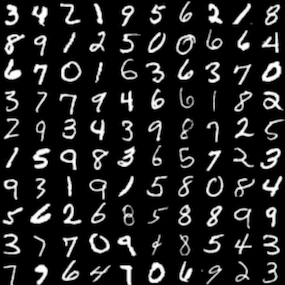
\includegraphics[width=\linewidth]{./Images/Chapter03/mnist_dataset.png}
  \endminipage\hfill
  \minipage{0.45\textwidth}%
    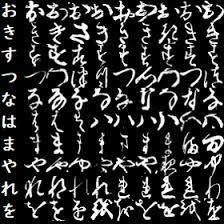
\includegraphics[width=\linewidth]{./Images/Chapter03/kuzushiji_mnist.jpg}
  \endminipage\hfill
  \caption{A visualization of two datasets that can be used for performing inductive transfer learning. On the left we represent instances of the popular MNIST dataset \cite{lecun1994mnist}, while on the right instances of the Kuzushiji-MNIST dataset \cite{clanuwat2018deep}. We see that both datasets share the same domain $\mathcal{D}_S = \mathcal{D}_T$ (black and white images), but are associated to different tasks $\mathcal{T}_S \neq \mathcal{T}_T$ (classification of digits vs classification of Japanese letters).}
  \label{fig:inductive_tl}
\end{figure*}


\paragraph{Transductive Transfer Learning}
Originally proposed by \citet{arnold2007comparative}, this type of TL is characterized by the fact that the source and target tasks are the same $\mathcal{T}_S = \mathcal{T}_T$, but their respective domains are different $\mathcal{D}_S \neq \mathcal{D}_T$. It is also possible that the feature spaces between domains are the same but, if that is the case, then the marginal probability distributions are different $P(X_S)\neq P(X_T)$. In its original formulation, \citet{arnold2007comparative} assumed that all unlabeled data in the target domain is available at training time, however we hereafter report the definition of \citet{pan2009survey} who instead relax this condition and require only a subset of unlabeled target data to be seen at training time.
\begin{definition}
	Given a source domain $\mathcal{D}_S$ and a learning task $\mathcal{T}_S$, and a target domain $\mathcal{D}_T$ and a learning task $\mathcal{T}_T$, transductive transfer learning aims to help improving the target predictive function $f_T(\cdot)$ in $\mathcal{D}_T$ by using the knowledge in $\mathcal{D}_S$ and $\mathcal{T}_S$, where $\mathcal{D}_S \neq \mathcal{D}_T$ and $\mathcal{T}_S = \mathcal{T}_T$. 
\end{definition}
As an example of transductive transfer learning let us assume that we would like to train a model to classify which type of clothing is depicted in an image. This time, differently from the inductive transfer learning case, the images in our target domain $\mathcal{D}_T$ are not black and white images anymore, but rather colored images, therefore they are defined over the RGB domain (see right image of Fig. \ref{fig:transductive_tl}). We now assume that we have access to a pre-trained model which has already been trained to classify the same type of clothes, with the main difference being that the images constituting the source domain $\mathcal{D}_S$ were black and white images (see left image of Fig. \ref{fig:transductive_tl}). If we now train this pre-trained model on our colored dataset we see that our setting fits the transductive transfer learning scenario: our considered domains are different $\mathcal{D}_S \neq \mathcal{D}_T$ (colored vs black and white images), but their respective tasks are the same  $\mathcal{T}_S \neq \mathcal{T}_T$, since a model is always trained to classify types of clothing.

\begin{figure*}
 \minipage{0.45\textwidth}
    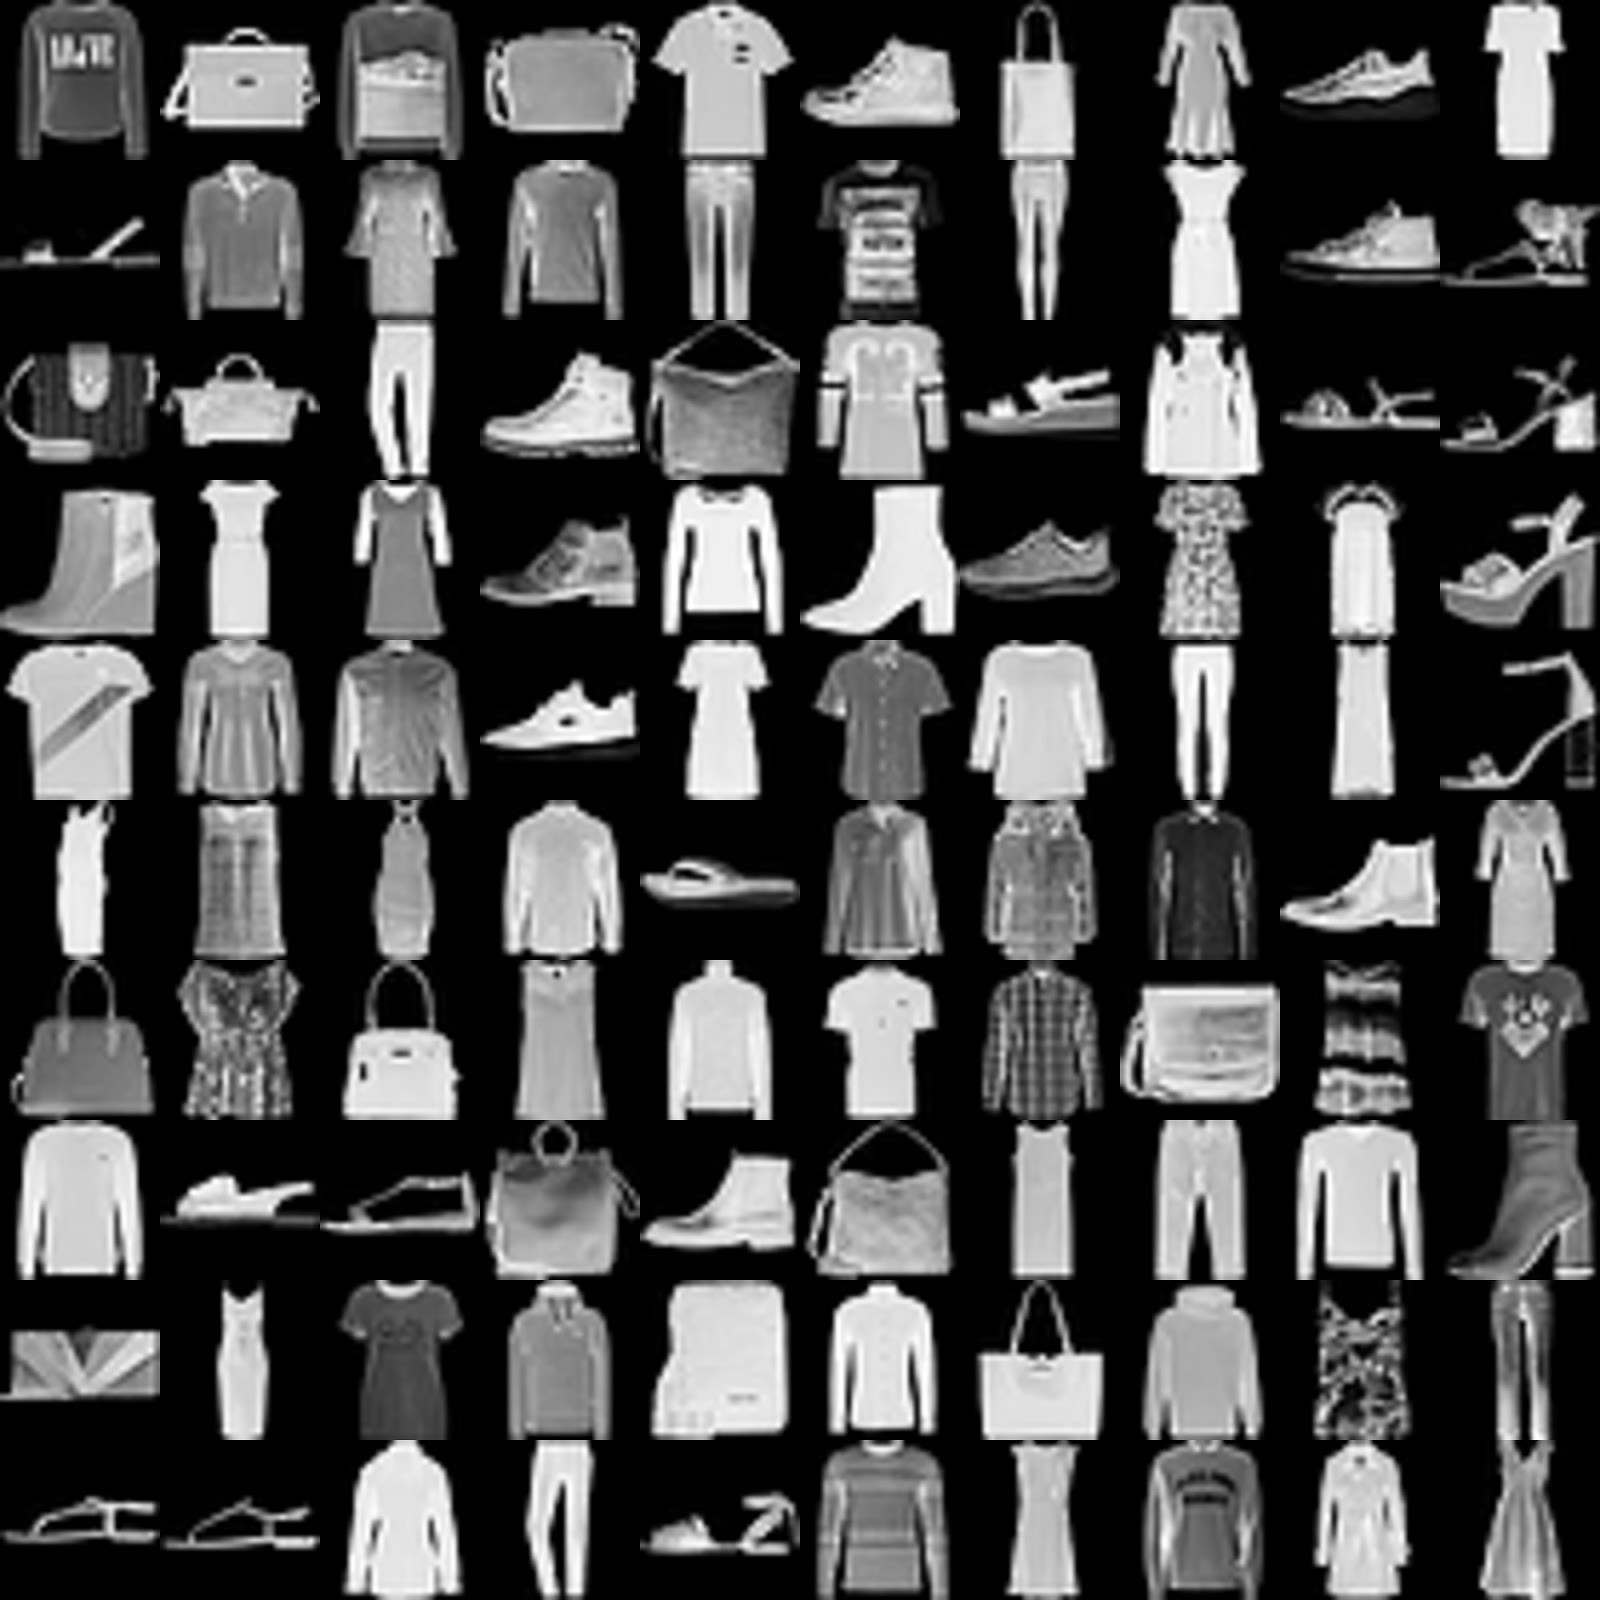
\includegraphics[width=\linewidth]{./Images/Chapter03/fashion_mnist}
  \endminipage\hfill
  \minipage{0.45\textwidth}%
    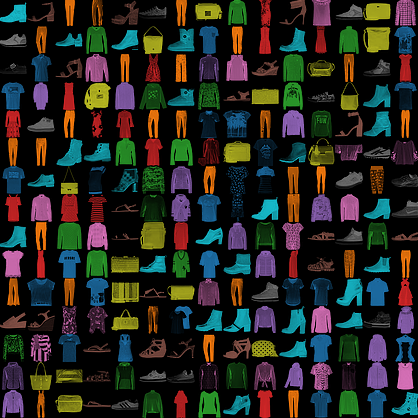
\includegraphics[width=\linewidth]{./Images/Chapter03/colorful_fashion_mnist}
  \endminipage\hfill
  \caption{Two datasets that are representative of transductive transfer learning. On the left we show images coming from the Fashion-MNIST dataset \cite{xiao2017fashion}, while on the right we report instances of the same dataset that are colored. In this case tasks among datasets are shared $\mathcal{T}_S = \mathcal{T}_T$ (classification of clothes), but the respective images come from different domains $\mathcal{D}_S \neq \mathcal{D}_T$ (black and white vs RGB images).}
  \label{fig:transductive_tl}
\end{figure*}

Although this section focuses on supervised learning, we still report for the sake of completeness a definition of unsupervised transfer learning hereafter, and see how this kind of TL is linked to the types of TL that we have analyzed so far

\paragraph{Unsupervised Transfer Learning}
Arguably considered to be the most challenging, and the least explored type of TL, unsupervised transfer learning is characterized by the total absence at training time of labeled data in both the source domain and the target domain. As mentioned by \citet{pan2009survey} very little research work has so far explored this TL paradigm, with the only existing works exploring typical unsupervised learning topics such as clustering \cite{dai2008self, jin2011transferring, qian2015cluster} and dimensionality reduction \cite{wang2008transferred, zhu2013self, zhu2016robust}. Unsupervised transfer learning is defined as follows:
\begin{definition}
	Given a source domain $\mathcal{D}_S$ and a learning task $\mathcal{T}_S$, and a target domain $\mathcal{D}_T$ and a learning task $\mathcal{T}_T$, unsupervised transfer learning aims to help improving the target predictive function $f_T(\cdot)$ in $\mathcal{D}_T$ by using the knowledge in $\mathcal{D}_S$ and $\mathcal{T}_S$, where $\mathcal{T}_S \neq \mathcal{T}_T$ and $\mathcal{Y}_S$ and $\mathcal{Y}_T$ are not observable. 
\end{definition}
Based on this definition we can note that unsupervised transfer learning is more similar to inductive transfer learning than to to transductive transfer learning since we again assume that the source and the target tasks are different $\mathcal{T}_S \neq \mathcal{T}_T$.


\subsection{Reinforcement Learning}
When it comes to the reinforcement learning setup, the aforementioned definition of TL slightly changes, and becomes arguably less general. Recall from Chapter \label{ch:reinforcement_learning} that in RL, the main goal is that of training an agent such that it becomes able to interact with its environment, a problem that is modeled with Markov Decision Process (MDP). It follows that in the RL context, the previously introduced concept of domain $\mathcal{D}$ (which could come in numerous flavors), now comes in the arguably more strictly defined form of a MDP $\mathcal{M}$. Just like domains, MDPs can either be representative of a source task, $\mathcal{M_S}$, or of a target $\mathcal{M}_T$ task, with the latter case corresponding to the main RL problem we are interested to solve. Also the previously introduced predictive function $f(\cdot)$ is now defined more precisely, since it corresponds to the task of learning an optimal policy $\pi^*$ for $\mathcal{M}_T$. Based on these concepts we give the following definition of TL for reinforcement learning that is adapted from the one proposed by \citet{zhu2020transfer}.

\begin{definition}
	Given a source MDP $\mathcal{M}_S$ and a target MDP $\mathcal{M}_D$, transfer learning in reinforcement learning aims to learn an optimal policy $\pi^{*}$ for $\mathcal{M}_D$ by exploiting some prior knowledge related to $\mathcal{M}_S$, $\mathcal{K}_S$, together with the knowledge that underlies $\mathcal{M}_T$, $\mathcal{K}_T$ such that:
	\begin{align}
		\pi^{*} = \argmax_{\pi} \mathds{E}_{s \sim\mu_{0}^{t},a\sim\pi}\bigl[Q^{\pi}_\mathcal{M}(s,a)\bigr],
	\end{align}
	where $\pi = \zeta(\mathcal{K}_S \sim \mathcal{M}_S, \mathcal{K}_T \sim \mathcal{M}_T): \mathcal{S}^t \rightarrow \mathcal{A}^t$ is a function mapping from the states to actions for $\mathcal{M}_T$ learned thanks to both $\mathcal{K}_S$ and $\mathcal{K}_T$.
\end{definition}

Note that differently from the supervised learning case we are now making explicit use of the concept of knowledge $\mathcal{K}$, which is what we would like to retain when moving from a source MDP $\mathcal{M}_S$ to a target MDP $\mathcal{M}_T$. We do this because RL is a machine learning paradigm that is, arguably, more complex than the supervised learning one. A complexity which stems from the fact that in RL there are concepts such as e.g. rewards and policies, which are, by definition, not present in the supervised learning setup. As a result, $\mathcal{K}$ can come in forms that it cannot take in SL, and correctly identifying which kind of knowledge to transfer between $\mathcal{M}_S$ and $\mathcal{M}_T$ is just as important as developing a method that successfully transfers this knowledge in the first place. As mentioned by \citet{lazaric2012transfer} and by \citet{tirinzoni2018transfer}, $\mathcal{K}$ can come in the following forms:

\paragraph{Transfer of Instances:} in this scenario $\mathcal{K}$ corresponds to RL trajectories coming in the form $\langle s_t, a_t, r_t, s_{t+1}\rangle$ and that have been collected on one, or possibly multiple, source MDPs $\mathcal{M}_S$. Such trajectories can then be used both in a model-based RL setting, as done by \citet{taylor2008transferring}, or for speeding up the process of learning a value function as described in \cite{lazaric2008transfer} and \cite{laroche2017transfer}. Ideally, transferring RL trajectories should result into algorithms that are highly sample efficient, although it is worth noting that this property, albeit desirable, can constrain the source task $\mathcal{M}_S$ and the target task $\mathcal{M}_T$ to have similar transition models and reward functions. This instance of TL is usually used within the batch RL setup, where gathering experience samples for $\mathcal{M}_T$ can be particularly expensive or time consuming, which is a constraint that, however does not hold for $\mathcal{M}_S$. The typical challenge is then correctly identifying which samples coming from $\mathcal{M}_S$ are the most informative ones for solving $\mathcal{M}_T$ \cite{tirinzoni2018importance}.

\paragraph{Transfer of Representations:}
\paragraph{Transfer of Parameters:}


\section{Deep Transfer Learning}
\label{sec:literature_review}

\subsection{General Framework}

\begin{itemize}
	\item \textcolor{RoyalBlue}{Off the Shelf Classification}
	\item \textcolor{RoyalBlue}{Fine-Tuning}
\end{itemize}


\subsection{Literature Review}
\paragraph{Supervised Learning} # not limited to vision ---> mention NLP, BERT, ...
\paragraph{Reinforcement Learning}

\section{Relevance for this Dissertation}
\label{sec:relevance}
